%%%%%%%%%%%%%%%%%%%%%%%%%%%%%%%%%%%%%%%%%
% Thesis LaTeX Template Modified by Ng for the Tesina Course
% Version 1.2 (05/24/2018)
% Note:
% Make sure to include the Thesis.cls  file in the folder
%%%%%%%%%%%%%%%%%%%%%%%%%%%%%%%%%%%%%%%%%

%----------------------------------------------------------------------------------------
%	PACKAGES AND OTHER DOCUMENT CONFIGURATIONS
%----------------------------------------------------------------------------------------

\documentclass[11pt, a4paper, oneside]{thesis} % paper size redifined in Thesis.cls
\usepackage[square, numbers, comma, sort&compress]{natbib}
\usepackage[nodayofweek]{datetime}
\usepackage{float}
\usepackage{color, colortbl}
\hyphenpenalty=10000
\renewcommand{\arraystretch}{1.25}
\definecolor{pale_yellow}{rgb}{1, 0.92, 0.673}
\definecolor{dark_blue}{rgb}{0.9, 0.9, 1}
\definecolor{blue}{rgb}{0.8, 0.8, 1}
\definecolor{light_blue}{rgb}{0.7, 0.7, 1}
\usepackage{array}
\usepackage{wrapfig}
\usepackage{pdfpages}
\usepackage[utf8]{inputenc}  % Ng Edit for accents in spanish
\usepackage[english]{babel}
\hypersetup{urlcolor=blue, colorlinks=false}
\title{\ttitle}
\thesistitle{tesina ISC}
\begin{document}
\frontmatter
\setstretch{1.3}

\fancyhead{}
\rhead{\thepage}
\lhead{}

\pagestyle{fancy}
\newcommand{\HRule}{\rule{\linewidth}{0.5mm}}

% PDF meta-data
\hypersetup{pdftitle={\ttitle}}
\hypersetup{pdfsubject=\subjectname}
%\hypersetup{pdfauthor=\authornames}
\hypersetup{pdfkeywords=\keywordnames}

%----------------------------------------------------------------------------------------
%	TITLE PAGE
%----------------------------------------------------------------------------------------

\begin{titlepage}
\begin{center}

\textsc{\Large \univname}\\
\textsc{\Large \facname}\\
\textsc{\Large \schoolname}\\[1cm]

\includegraphics[scale=.3]{logo.png} \\
\centering{\Large \bfseries Spanish Resumes Named Entity Recognition with \\
Conditional Random Fields}\\[0.5cm]

\large by\\[0.5cm]

\begin{minipage}{0.4\textwidth}
\begin{center} \large
\authors{Juan Alejandro Alcántara Minaya}
\large{\href{mailto:A01703947@exatec.tec.mx?subject=Awesome thesis, man!}{\authornames}} 
\\[0.5cm] 
\end{center}
\end{minipage}\\[0.5cm]

\large Proyecto Integrador para el Desarrollo de Soluciones Empresariales \\ \textit{\degreename}\\[0.8cm]

\begin{table}[!h]
\begin{center}
\begin{tabular}{lll}
\multicolumn{1}{r}{Advisor:} & Dr. Benjamín Valdés \\  %modificame nombre de tu asesor
\end{tabular}
\end{center}
\end{table}

\vspace{3cm}
Santiago de Querétaro, Querétaro, México \\

{\large \longdate{08/06/2022}}\\[1.5cm]%modificame fecha de la tesina
%This document represents a work in progress. The statements and information reported here \textit{may be} artistic works of fiction and fantasy.
\vfill
\end{center}

\end{titlepage}


\clearpage % Start a new page

%----------------------------------------------------------------------------------------
%	QUOTATION PAGE
%----------------------------------------------------------------------------------------

\pagestyle{empty} % No headers or footers for the following pages%
\null\vfill

\begin{center}
\textit{"Some people call this artificial intelligence, but the reality is this
technology will enhance us. So instead of artificial intelligence, I think
we’ll augment our intelligence."}
\end{center}

\begin{flushright}
Ginni Rometty
\end{flushright}

\vfill\vfill\vfill\vfill\vfill\vfill\null 

\clearpage


%----------------------------------------------------------------------------------------
%	ACKNOWLEDGEMENTS
%----------------------------------------------------------------------------------------

\setstretch{1.3} % Reset the line-spacing to 1.3 for body text (if it has changed)

\acknowledgements{\addtocontents{toc}{\vspace{1em}}  %modificame tus agradecimientos van aquí solo si quieres sino puedes borrar la sección
This thesis is the culmination of years of hard work, difficult decisions,
and obstacles on the road. I must thank the people that helped me through it
and immortalize them for their contributions.
\vskip 30pt

I thank all my teachers and staff members at ITESM for creating a learning
environment where I could learn from my mistakes and grow stronger along with
my peers. Thank you for not giving up on your students.
\vskip 30pt

I thank my friends and family for all the sweat and tears shared to get me to
where I am today. Thank you for letting me talk your ears off about my niche
topics and for supporting my dreams. Thank you, Carmelina and Paty, for all
your hard work put into this thesis.
\vskip 30pt

Finally, I would like to thank my father for teaching me the value of a
fulfilling education, what are the priorities in life, and the values that
maketh a man.
}
\clearpage % Start a new page


%----------------------------------------------------------------------------------------
%	ABSTRACT PAGE
%----------------------------------------------------------------------------------------

\addtotoc{Abstract} % Add the "Abstract" page entry to the Contents

 

\abstract{\addtocontents{toc}{\vspace{1em}} %modificame 
	With the growth of the digital age, many traditional recruiting methods are
	becoming obsolete. Long gone are the days when you would walk up to an office
	and deposit your printed-out resumes. Today, resumes are submitted digitally
	through a myriad of different platforms. With the ease of submission came the
	volume growth. As a result, we have developed tools to help recruiters parse
	through the large pool of candidates. Researchers created these tools for the
	English language; however, much remains to be done for Spanish. Our objective
	is to build an automated tool that helps recruiters extract essential
	information from a resume and reduce the amount of data. We based our
	approach on the Conditional Random Fields probabilistic model. We tested
	three different feature sets against a small sample of Spanish resumes and
	discovered riveting data patterns. These findings helped us generate a
	contribution to the field, and at the end of this paper, we explore its
	implications.

\clearpage

%----------------------------------------------------------------------------------------
%	LIST OF CONTENTS/FIGURES/TABLES PAGES
%----------------------------------------------------------------------------------------

\pagestyle{fancy}

%\lhead{\emph{List of Figures}} % Set the left side page header to "List of Figures"
%\listoffigures % Write out the List of Figures

%\lhead{\emph{List of Tables}} % Set the left side page header to "List of Tables"
%\listoftables % Write out the List of Tables

\lhead{\emph{Contents}} % Set the left side page header to "Contents"
\tableofcontents % Write out the Table of Contents

%----------------------------------------------------------------------------------------
%	ABBREVIATIONS
%----------------------------------------------------------------------------------------

\clearpage
\setstretch{1.5}

\lhead{\emph{Acronyms}} % Set the left side page header to "Abbreviations"
\listofsymbols{ll} % Include a list of Abbreviations (a table of two columns)
{
\textbf{NLP} & \textbf{N}atural \textbf{L}anguage \textbf{P}rocessing \\
\textbf{NER} & \textbf{N}amed \textbf{E}ntity \textbf{R}ecognition \\
\textbf{CRF} & \textbf{C}onditional \textbf{R}andom \textbf{F}ields \\
\textbf{HMM} & \textbf{H}idden \textbf{M}arkov \textbf{M}odels \\
\textbf{POS} & \textbf{P}art \textbf{O}f \textbf{S}peech \\
}

%----------------------------------------------------------------------------------------
%	PHYSICAL CONSTANTS/OTHER DEFINITIONS
%----------------------------------------------------------------------------------------

%\clearpage

%\lhead{\emph{Physical Constants}} % Set the left side page header to "Physical Constants"

%\listofconstants{lrcl} % Include a list of Physical Constants (a four column table)
%{
%Speed of Light & $c$ & $=$ & $2.997\ 924\ 58\times10^{8}\ \mbox{ms}^{-\mbox{s}}$ (exact)\\
%}

%----------------------------------------------------------------------------------------
%	SYMBOLS
%----------------------------------------------------------------------------------------

%\clearpage

%\lhead{\emph{Variables and Symbols}} % Set the left side page header to "Symbols"

%\listofnomenclature{lll} % Include a list of Symbols (a three column table)
%{
%$a$ & distance & m \\
%$P$ & power & W (Js$^{-1}$) \\
% Symbol & Name & Unit \\

%& & \\ % Gap to separate the Roman symbols from the Greek

%$\omega$ & angular frequency & rads$^{-1}$ \\
% Symbol & Name & Unit \\
%}

%----------------------------------------------------------------------------------------
%	THESIS CONTENT - CHAPTERS
%----------------------------------------------------------------------------------------

\mainmatter % Begin page numbering

\pagestyle{fancy}

% Include the chapters of the thesis as separate files from the Chapters folder

% Capítulo 1

\chapter{Introduction} % Main chapter title

\label{Cap1} % For referencing the chapter elsewhere, use \ref{Chapter1} 

\lhead{Capítulo 1. \emph{Introduction}} % This is for the header on each page - perhaps a shortened title

  We are often faced with the debate of humans versus machines, with a lot of
  people concerned that they will be replaced by robots. However, the goal has
  always been to strengthen the relationship between automated systems and
  humans to improve the overall work quality. The objective of this research
  paper is to provide an automated tool to help Spanish recruiters parse
  through the large volume of resumes they handle daily.

  There are a lot of existing tools that help recruiters in other languages,
  such as English, to process candidate resumes. Most commonly known as
  Applicant Tracking Systems (ATS), these systems help filter through a pool of
  candidates and provide the best match for a job vacancy. However, these tools
  are not as widespread in the Spanish language. We decided to take on the
  challenge of creating something similar to help the development of
  the area.

  More significantly, we focused on developing a said tool using a lesser-known
  type of model called Conditional Random Fields (CRF) since it offers great
  benefits at low computational costs. Other research has shown how these
  models compare to traditional deep learning methods and it shows a lot of
  promise. The biggest challenge, however, is being able to capture and convey
  the nuances of Spanish resumes so that a model can understand how to process
  them.

  Building tools like this one don't have the objective of displacing people
  from their jobs, but instead of freeing up their time and effort toward more
  rewarding tasks. Processing large datasets can be tolling for humans and the
  best way to combat it is with the help of machines. The future of work is
  pointed toward collaboration with automated systems and we strive to be part
  of it.



% Capítulo 2

\chapter{State of the Art} % Main chapter title

\label{Cap2}

\lhead{Capítulo 2. \emph{State of the Art}} % This is for the header on each page - perhaps a shortened title

This chapter focuses on establishing the knowledge base necessary to understand
the solution and design choices that come with it. Based on these concepts and
previous work, we can then address what to do to contribute to the status quo.

\section{Literature Review}
  \subsection{Named Entity Recognition (NER)}
  Named Entity Recognition is a subarea of Natural Language Processing. Its
  objective is to locate and categorize important words in a text. This process
  is crucial in applications that focus on information extraction, translation,
  and overall text analysis. Usually, named entities are classified according
  to the information they provide. For example, NER tasks frequently focus on
  extracting people, locations, and organizations from large text corpora
  \cite{Mohit2014}.

  There are two main challenges in named entity recognition tasks. The first
  one is determining the correct boundaries for a certain entity and the second
  one is determining the correct class for said entity. The author explains
  that there are ambiguous examples where it is easy for the models to make a
  mistake. For instance, the word \textit{Fox} can be interpreted as either a
  person or an organization. Another challenge arises when you consider that
  different domains consider different entities essential. For example, in
  resumes, the word \textit{Python} can refer to a skill, whereas in biology it
  may be referring to an animal. It is, therefore, crucial to have specifically
  labeled corpora tailored for the specific domain. \cite{Mohit2014}

  \subsection{Conditional Random Fields (CRF)}
  Conditional Random Fields are undirected probabilistic graphical models
  that tackle sequence analysis. It is often confused with Hidden Markov Models
  (HMMs) since they share some similarities. However, the main difference is
  that HMMs are a form of generative model and to "define a joint
  distribution... [it] must enumerate all possible observation sequences
  - a task which... is intractable unless observation elements are
  represented as isolated units" \cite{Wallach2004}.

  Nonetheless, Conditional Random Fields can model the dependency between
  different observations without having to increase model complexity. This
  property also allows the model to consider past and future tokens for the
  probabilistic prediction of the current token \cite{Lafferty2001}.
  \begin{figure}[ht!]
    \centering
    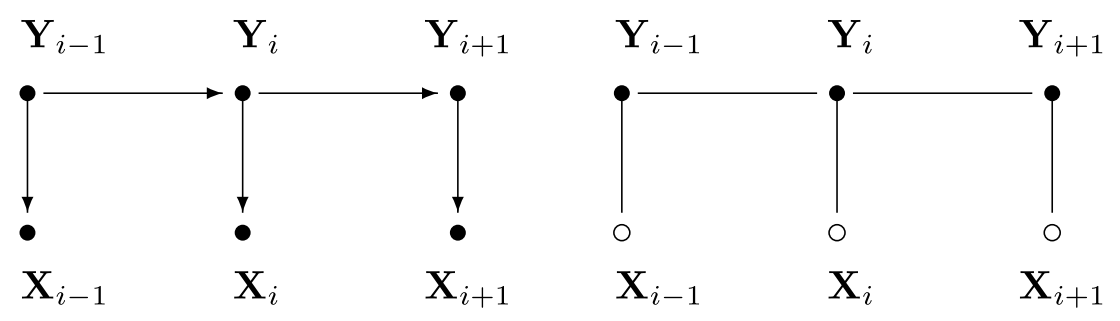
\includegraphics[width=\columnwidth]{hmm_vs_crf.png}
    \caption{%
      Graphical structures of simple HMMs (left), and chain-structured case of
      CRFs (right) for sequences. An open circle indicates that the variable is
      not generated by the model. \cite{Lafferty2001}
    }
  \end{figure}
  With CRFs, you can manually select the features that better suit your
  problem. For instance, if we were using CRFs to extract contact information
  from a corpus of text, we can choose specific format characteristics of
  sequences like phone numbers, emails, and websites to improve its
  performance. This flexibility makes this model attractive as an
  out-of-the-box solution to previously tackled problems.

\clearpage
\section{Related Work}

  Resumes fall into the category of semi-structured documents. This
  characteristic poses a challenge for traditional parsing methods because the
  contents, although usually grouped by topic, do not share a single format.
  Computer scientists have had to rely on natural language processing (NLP)
  techniques to extract the relevant content. Different authors have used part
  of speech (POS) tagging, \textit{stop word} removal, and stemming to process
  the resume text content \cite{Sanyal2015,Ayishathahira2018a,Roy2020a}.

  \subsection{English Resume Parsing}
  Roy et al. \cite{Roy2020a} performed another survey of different classifier
  models such as Random Forests, Multinomial Naive Bayes, Logistic Regression,
  and Linear Support Vector Machines (LSVM). Their objective was to classify
  resumes into different job sectors such as sales, consulting, finance,
  technology, etc. To feed the data into the models they had to remove junk
  characters, and \textit{stop words} from the resumes. They also had to use
  stemming and lemmatization. This led to data loss, which is mentioned in the
  limitations. However, their objective was not to gather the specifics of
  their resumes, but instead to get a general idea of the candidate profile.
  Their research showed that the most performant model was the LSVM, with an
  average accuracy of 78.53\%.

  This survey showcases that for resume parsing the best model is usually the
  model that excels at sequence analysis. It shouldn't come as a surprise since
  resumes are semi-structured documents.

  \medskip
  On this note, Ayishathahira et al. \cite{Ayishathahira2018a} focused on
  effectively gathering named entities by comparing the performance of four
  models:
  \begin{itemize}
    \item Convolutional Neural Network (CNN)
    \item Bidirectional Long Short-Term Memory (Bi-LSTM)
    \item Conditional Random Field (CRF)
    \item Bi-LSTM and CNN combination (Bi-LSTM-CNN)
  \end{itemize}
  They worked with a dataset of 800 resumes sourced privately by one of their
  sponsors. They removed punctuations and other extraneous characters as well.
  Nevertheless, the authors didn't use lemmatization or stemming which allowed
  the sequences to remain mostly intact.

  Ayishathahira et al. defined 23 labels to classify information about a
  candidate's education, occupation, and identification. They trained the
  models to discover that the CRF implementation yielded the best results. On
  average, the CRF model had an F-score of 83.70\% while the Bi-LSTM-CNN had an
  F-score of 68.43\%. The CRF model beat the Bi-LSTM-CNN model across all the
  labels, with an average improvement of 15.26\%.

  The CRF model showed great advantages over its counterparts. It is relatively
  fast to train, needing less than half an hour to go through the authors'
  dataset. This speed, combined with its accuracy, makes the CRF model a great
  candidate to develop effective resume parsing tools.

  \medskip
  E. Suhas and E. Manjunath \cite{E*2020} took Ayishathahira's
  \cite{Ayishathahira2018a} research even further and they were able to develop
  a mixed model that allowed them to match candidates with job postings. The
  model is a combination of Named Entity Recognition (NER) and Word2Vec
  embedding to find the cosine distance between entities in resumes and job
  postings.

  They generated four different iterations of the NER model using, Stanford's
  NER model as a basis. They either removed more noise or increased the dataset
  size on each iteration and this translated to an F-score increase from about
  52\% to more than 80\%. The largest increase, of about 15\%, was achieved
  from the third iteration to the fourth iteration by introducing a dictionary
  of technical skills to the NER and increasing the window size.

  Even though this study had a smaller dataset than Ayishathahira's
  \cite{Ayishathahira2018a}, they were able to achieve similar results. Since
  it is a time-consuming and arduous process to prepare these datasets, this
  strategy is a great alternative to get the most out of the available
  resources.

  \subsection{Spanish Named Entity Recognition}
  Based on the research done for English corpus, Copara et al.
  \cite{Copara2016} developed a model that allowed named entity recognition for
  Spanish text. They decided to evaluate their model by using the CoNLL-2002
  (Spanish) dataset since it allows them to compare their performance against
  the state of the art.

  The authors decided to use word embedding and clustering in hopes of
  achieving better results. They used a large corpus of text both in Spanish
  and English to generate robust embeddings. Their baseline model achieved an
  F-score of 80.02\%. After adding embedding and clustering, they were able to
  increase this score to 82.30\%. They noticed that there are words that are
  more likely to belong to one class than to another class and decided to use
  distributional prototypes to leverage this pattern. After adding prototypes,
  the model's F-score dropped to 81.19\%. Nevertheless, they had the hypothesis
  that some entities share very similar features across languages and decided
  to use the Brown clusters from English. The model's F-score increased to
  82.44\%.

  Although the study didn't cover resumes specifically, it showcased various
  strategies to get better performance, even with a Spanish dataset. The most
  impressive observation is that the CRF model performed very similarly to the
  current state-of-the-art deep learning models.

\section{Why Conditional Random Fields in Spanish?}
The most relevant work to our research is Ayishathahira et al.
\cite{Ayishathahira2018a} and Copara et al. \cite{Copara2016} since they merge
the tools we need to address our problem. The former compares traditional
time-consuming extraction methods and flexible probabilistic models and
concluded that these models were better. The latter showed no special
considerations when working with named entity recognition in Spanish.
Therefore, we hypothesize that combining the language and the approach will
yield relevant results.

\section{Conclusion}
There is a lot of research on extracting the essential information from text,
especially from resumes. Regardless of the method chosen, it is vital to
develop tools to obtain this information in Spanish. Resumes are generally
universal documents, and the same techniques applied to English benefit
applications in other languages. We gathered the necessary knowledge to address
the problem ahead.


% Capítulo 3

\chapter{Problem Statement} % Main chapter title

\label{Cap3} % For referencing the chapter elsewhere, use \ref{Chapter1} 

\lhead{Capítulo 3. \emph{Problem Statement}} % This is for the header on each page - perhaps a shortened title
  Considering the relevant work, we have to put the problem into perspective.
  According to the Economic Commission for Latin America and the Caribbean
  (ECLAC), in 2019, an estimated average of 3.8 million workers searched for
  work daily \cite{Hilbert2020a}. The same report estimated a daily average of
  1.4 million job offer calls \cite{Hilbert2020a}. The supply is almost three
  times the demand, and it presents itself as an unmanageable task for
  recruiters across the region. Finding the best employee for a position is
  time-consuming since it requires combing through many candidates, and often
  missing essential information.

  It is crucial to act now since we are seeing an uptick in job
  applications. We are still experiencing the post-pandemic effects on the
  economy. In December 2021, the U.S. Bureau of Labor Statistics reported the
  lowest unemployment rate, 3.9\%, since January 2001 \cite{Kurt2022}. People
  had to change jobs due to layoffs and better opportunities. Nonetheless, this
  wasn't enough time for companies to update their recruiting methods.

  \vskip 35pt
  The problem is that, while in English-speaking countries there are tools to
  aid companies to handle the sheer volume of applications, there are not
  enough of these tools for Spanish-speaking countries.


% Capítulo 4

\chapter{Solution} % Main chapter title

\label{Cap4} % For referencing the chapter elsewhere, use \ref{Chapter1} 

\lhead{Capítulo 4. \emph{Solution}} % This is for the header on each page - perhaps a shortened title

  The most viable solution to this problem is using Conditional Random Fields
  (CRF) to extract the essential information from candidates' resumes. Compared
  to the training time and complexity of deep learning methods, CRFs are
  quicker and simpler to implement. The key to building a robust CRF is
  choosing the right features and having a large enough dataset. In comparison,
  Conditional Random Fields are more flexible allowing the model to find
  relationships between sequences even if they are not immediately next to each
  other. These characteristics and the research so far suggest that these
  models will yield good results when parsing resumes, regardless of the
  language.

  We discussed with an HR representative what information would be the most
  relevant to choosing a candidate. Based on her answers, we defined 13
  categories to classify the resume information. These categories comprise
  things like the candidate's names, experience, and education. This is the
  list of classes defined in conjunction with the recruiter:
  \begin{itemize}
    \item \textbf{Company}: The institutions the candidate has worked for
    \item \textbf{Degree}: The education the candidate has received
    \item \textbf{Designation}: The job positions the candidate has occupied
    \item \textbf{Email}: The candidate's contact email
    \item \textbf{End Date}: When the candidate was done with either a job
      position or a degree
    \item \textbf{First Name}: The candidate's first name
    \item \textbf{Last Name}: The candidate's last name
    \item \textbf{Location}: A physical address or city/state/country
    \item \textbf{Phone Number}: The candidate's phone number
    \item \textbf{School}: The education institution at which the candidate
      completed a degree
    \item \textbf{Skill}: A specific ability or skill acquired by the candidate
    \item \textbf{Start Date}: When the candidate started a job position or a
      degree
  \end{itemize}

  It is difficult to settle on a fixed sequence size to analyze each step of
  the CRF training. Depending on the field, the candidate, and the template,
  sequences for the same data can vary greatly. Traditionally, other
  researchers have used a word per word basis to train their models
  \cite{Ayishathahira2018a,E*2020}. Having settled on this strategy, we
  built three different feature sets (see \ref{table:1}, \ref{table:2}, and
  \ref{table:3}) to train the CRF.

  We built the solution using the Python library, \texttt{sklearn-crfsuite}
  version 0.3.6 which is a \texttt{scikit-learn} compatible wrapper for the C++
  library \texttt{CRFSuite} \cite{CRFsuite}. The library allows its users to
  create linear-chain CRFs using multiple training methods such as
  Limited-memory BFGS (L-BFGS), Stochastic Gradient Descent (SDG), Adaptive
  Regularization Of Weight Vector (AROW), etc. For this solution, we went with
  L-BFGS since it allowed us to set L1 and L2 normalization parameters.

  Before inputting the resumes into the model, we must convert them from their
  original file format to plain text. This process is challenging because some
  file formats, like PDFs, don't have a single way to parse them. After
  evaluating different options, we settled on using \texttt{pdfminer.six}
  version 20220524. This Python library correctly parsed most of our dataset.

  After having designed the model and converted the documents, we added
  preprocessing steps to feed it data. We parsed each resume into word tokens,
  eliminating common punctuation points such as periods, commas, question
  marks, etc. The next step was to calculate the features for each word in the
  resume as described in the tables (\ref{table:1}, \ref{table:2},
  \ref{table:3}). It is important to note that for the first and last word of
  each sequence features belonging to the previous and next word, respectively,
  were omitted.

  \begin{figure}[H]
    \centering
    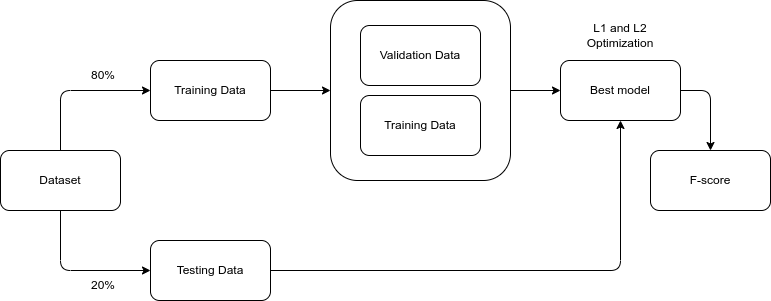
\includegraphics[width=\columnwidth]{model_training_process.png}
    \caption{%
      General process for training and testing
    }
  \end{figure}

  CRFs are great to predict what is the most likely transition from one
  tag to another, which is why they are an attractive solution to analyze
  semi-structured documents such as resumes. Based on this fact and the
  existing research so far, we believe this is a sufficient solution to address
  the problem at hand.

  \begin{table}[ht]
    \centering
    \begin{tabular}{|p{0.3\linewidth}|p{0.6\linewidth}|}
      \hline
      \textbf{Feature} & \textbf{Description} \\
      \hline
      \rowcolor{dark_blue}
      -1:word.istitle & Whether the previous word starts with a capital letter.
      \\
      \hline
      \rowcolor{dark_blue}
      -1:word.isdigit & Whether the previous word is an integer. \\
      \hline
      \rowcolor{dark_blue}
      -1:word.is\_year & Whether the previous word is an integer between 1900
      and 2100 (inclusive). \\
      \hline
      \rowcolor{dark_blue}
      -1:word.is\_abbr\_month & Whether the previous word is a month's name
      abbreviation. \\
      \hline
      \rowcolor{dark_blue}
      -1:word.is\_full\_month & Whether the previous word is a month's name. \\
      \hline
      \rowcolor{dark_blue}
      -1:word.syllable\_count & How many syllables does the previous word have,
      based on its vowels. \\
      \hline
      \rowcolor{dark_blue}
      -1:word.lower & The full previous word in lowercase. \\
      \hline
      \rowcolor{dark_blue}
      -1:word.bigram & The previous word concatenated with the current word. \\
      \hline
      \rowcolor{blue}
      word.istitle & Whether the current word starts with a capital letter. \\
      \hline
      \rowcolor{blue}
      word.isdigit & Whether the current word is an integer.\\
      \hline
      \rowcolor{blue}
      word.is\_year & Whether the current word is an integer between 1900
      and 2100 (inclusive). \\
      \hline
      \rowcolor{blue}
      word.len & Then length of the current word \\
      \hline
      \rowcolor{blue}
      word.is\_abbr\_month & Whether the current word is a month's name
      abbreviation. \\
      \hline
      \rowcolor{blue}
      word.is\_full\_month & Whether the current word is a month's name. \\
      \hline
      \rowcolor{blue}
      word.syllable\_count & How many syllables does the current word have,
      based on its vowels. \\
      \hline
      \rowcolor{blue}
      word.has\_at & Whether the current word has an @ symbol. \\
      \hline
      \rowcolor{light_blue}
      +1:word.istitle & Whether the next word starts with a capital letter. \\
      \hline
      \rowcolor{light_blue}
      +1:word.isdigit & Whether the next word is an integer. \\
      \hline
      \rowcolor{light_blue}
      +1:word.is\_year & Whether the current word is an integer between 1900
      and 2100 (inclusive). \\
      \hline
      \rowcolor{light_blue}
      +1:word.is\_abbr\_month & Whether the next word is a month's name
      abbreviation. \\
      \hline
      \rowcolor{light_blue}
      +1:word.is\_full\_month & Whether the next word is a month's name. \\
      \hline
      \rowcolor{light_blue}
      +1:word.syllable\_count & How many syllables does the current word have,
      based on its vowels. \\
      \hline
      \rowcolor{light_blue}
      +1:word.lower & The full next word in lowercase. \\
      \hline
      \rowcolor{light_blue}
      +1:word.bigram & The current word concatenated with the next word. \\
      \hline
    \end{tabular}
    \caption{Baseline Features}
    \label{table:1}
  \end{table}

  \clearpage
  \begin{table}[ht]
    \centering
    \begin{tabular}{|p{0.3\linewidth}|p{0.7\linewidth}|}
      \hline
      \textbf{Feature} & \textbf{Description} \\
      \hline
      \rowcolor{dark_blue}
      -1:word.istitle & Whether the previous word starts with a capital letter.
      \\
      \hline
      \rowcolor{dark_blue}
      -1:word.isdigit & Whether the previous word is an integer. \\
      \hline
      \rowcolor{dark_blue}
      -1:word.is\_year & Whether the previous word is an integer between 1900
      and 2100 (inclusive). \\
      \hline
      \rowcolor{dark_blue}
      -1:word.is\_abbr\_month & Whether the previous word is a month's name
      abbreviation. \\
      \hline
      \rowcolor{dark_blue}
      -1:word.is\_full\_month & Whether the previous word is a month's name. \\
      \hline
      \rowcolor{dark_blue}
      -1:word.syllable\_count & How many syllables does the previous word have,
      based on its vowels. \\
      \hline
      \rowcolor{dark_blue}
      -1:word.lower & The full previous word in lowercase. \\
      \hline
      \rowcolor{dark_blue}
      -1:word.bigram & The previous word concatenated with the current word. \\
      \hline
      \rowcolor{pale_yellow}
      -1:word.first\_three & The previous word first three characters \\
      \hline
      \rowcolor{pale_yellow}
      -1:word.last\_three & The previous word last three characters. \\
      \hline
      \rowcolor{blue}
      word.istitle & Whether the current word starts with a capital letter. \\
      \hline
      \rowcolor{blue}
      word.isdigit & Whether the current word is an integer. \\
      \hline
      \rowcolor{blue}
      word.is\_year & Whether the current word is an integer between 1900
      and 2100 (inclusive). \\
      \hline
      \rowcolor{blue}
      word.len & Then length of the current word \\
      \hline
      \rowcolor{blue}
      word.is\_abbr\_month & Whether the current word is a month's name
      abbreviation. \\
      \hline
      \rowcolor{blue}
      word.is\_full\_month & Whether the current word is a month's name. \\
      \hline
      \rowcolor{blue}
      word.syllable\_count & How many syllables does the current word have,
      based on its vowels. \\
      \hline
      \rowcolor{blue}
      word.has\_at & Whether the current word has an @ symbol. \\
      \hline
      \rowcolor{pale_yellow}
      word.first\_three & The current word first three characters \\
      \hline
      \rowcolor{pale_yellow}
      word.last\_three & The current word last three characters. \\
      \hline
      \rowcolor{light_blue}
      +1:word.istitle & Whether the next word starts with a capital letter. \\
      \hline
      \rowcolor{light_blue}
      +1:word.isdigit & Whether the next word is an integer. \\
      \hline
      \rowcolor{light_blue}
      +1:word.is\_year & Whether the current word is an integer between 1900
      and 2100 (inclusive). \\
      \hline
      \rowcolor{light_blue}
      +1:word.is\_abbr\_month & Whether the next word is a month's name
      abbreviation. \\
      \hline
      \rowcolor{light_blue}
      +1:word.is\_full\_month & Whether the next word is a month's name. \\
      \hline
      \rowcolor{light_blue}
      +1:word.syllable\_count & How many syllables does the current word have,
      based on its vowels. \\
      \hline
      \rowcolor{light_blue}
      +1:word.lower & The full next word in lowercase. \\
      \hline
      \rowcolor{light_blue}
      +1:word.bigram & The current word concatenated with the next word. \\
      \hline
      \rowcolor{pale_yellow}
      +1:word.first\_three & The next word first three characters \\
      \hline
      \rowcolor{pale_yellow}
      +1:word.last\_three & The next word last three characters. \\
      \hline
    \end{tabular}
    \caption{Head + Tail \\ \textnormal{(Changes marked in yellow)}}
    \label{table:2}
  \end{table}

  \begin{table}[pt]
    \centering
    \begin{tabular}{|p{0.3\linewidth}|p{0.6\linewidth}|}
      \hline
      \textbf{Feature} & \textbf{Description} \\
      \hline
      \rowcolor{dark_blue}
      -1:word.istitle & Whether the previous word starts with a capital letter.
      \\
      \hline
      \rowcolor{dark_blue}
      -1:word.isdigit & Whether the previous word is an integer. \\
      \hline
      \rowcolor{dark_blue}
      -1:word.is\_year & Whether the previous word is an integer between 1900
      and 2100 (inclusive). \\
      \hline
      \rowcolor{dark_blue}
      -1:word.is\_abbr\_month & Whether the previous word is a month's name
      abbreviation. \\
      \hline
      \rowcolor{dark_blue}
      -1:word.is\_full\_month & Whether the previous word is a month's name. \\
      \hline
      \rowcolor{dark_blue}
      -1:word.syllable\_count & How many syllables does the previous word have,
      based on its vowels. \\
      \hline
      \rowcolor{dark_blue}
      -1:word.lower & The full previous word in lowercase. \\
      \hline
      \rowcolor{dark_blue}
      -1:word.bigram & The previous word concatenated with the current word. \\
      \hline
      \rowcolor{dark_blue}
      -1:word.first\_three & The previous word first three characters \\
      \hline
      \rowcolor{dark_blue}
      -1:word.last\_three & The previous word last three characters. \\
      \hline
      \rowcolor{blue}
      word.istitle & Whether the current word starts with a capital letter. \\
      \hline
      \rowcolor{blue}
      word.isdigit & Whether the current word is an integer. \\
      \hline
      \rowcolor{blue}
      word.is\_year & Whether the current word is an integer between 1900
      and 2100 (inclusive). \\
      \hline
      \rowcolor{blue}
      word.len & Then length of the current word \\
      \hline
      \rowcolor{blue}
      word.is\_abbr\_month & Whether the current word is a month's name
      abbreviation. \\
      \hline
      \rowcolor{blue}
      word.is\_full\_month & Whether the current word is a month's name. \\
      \hline
      \rowcolor{blue}
      word.syllable\_count & How many syllables does the current word have,
      based on its vowels. \\
      \hline
      \rowcolor{blue}
      word.has\_at & Whether the current word has an @ symbol. \\
      \hline
      \rowcolor{blue}
      word.first\_three & The current word first three characters \\
      \hline
      \rowcolor{blue}
      word.last\_three & The current word last three characters. \\
      \hline
      \rowcolor{pale_yellow}
      word.lower & The full current word in lowercase. \\
      \hline
      \rowcolor{light_blue}
      +1:word.istitle & Whether the next word starts with a capital letter. \\
      \hline
      \rowcolor{light_blue}
      +1:word.isdigit & Whether the next word is an integer. \\
      \hline
      \rowcolor{light_blue}
      +1:word.is\_year & Whether the current word is an integer between 1900
      and 2100 (inclusive). \\
      \hline
      \rowcolor{light_blue}
      +1:word.is\_abbr\_month & Whether the next word is a month's name
      abbreviation. \\
      \hline
      \rowcolor{light_blue}
      +1:word.is\_full\_month & Whether the next word is a month's name. \\
      \hline
      \rowcolor{light_blue}
      +1:word.syllable\_count & How many syllables does the current word have,
      based on its vowels. \\
      \hline
      \rowcolor{light_blue}
      +1:word.lower & The full next word in lowercase. \\
      \hline
      \rowcolor{light_blue}
      +1:word.bigram & The current word concatenated with the next word. \\
      \hline
      \rowcolor{light_blue}
      +1:word.first\_three & The next word first three characters \\
      \hline
      \rowcolor{light_blue}
      +1:word.last\_three & The next word last three characters. \\
      \hline
    \end{tabular}
    \caption{Whole Word \\ \textnormal{(Changes marked in yellow)}}
    \label{table:3}
  \end{table}




% Capítulo 5

  \chapter{Experimentation \& Evaluation} % Main chapter title

\label{Cap5} % For referencing the chapter elsewhere, use \ref{Chapter1} 

\lhead{Capítulo 5. \emph{Experimentation \& Evaluation}} % This is for the header on each page - perhaps a shortened title
  There is a lack of public Spanish datasets with tagged resumes, which meant
  that we had to gather and build our own. First, we needed to collect
  Spanish resumes and convert them from their original formats to plain text.
  This can be challenging due to the great diversity of file formats and resume
  templates. Building a named entity recognition dataset is a laborious
  task since it means going through each data sample and labeling the sequences
  by hand. We were able to accomplish this task thanks to the open-source
  program, Doccano. Doccano provides a graphical interface to label the
  documents by selecting the text and assigning a label. After labeling each
  resume, we used the dataset to train the model and evaluate its performance.

  We collected resumes from two main sources: an HR representative at an
  automotive manufacturing company and Mexico's government representatives'
  public available resumes. In total, we collected over 90 resumes, of which we
  could only use 51 due to errors in the text conversion. The resumes comprised
  different profiles such as engineers, marketers, lawyers, educators, and
  public servants. Although it would have been ideal to have a larger dataset,
  we were limited by the available time and resources.

  The dataset was split in a 1:5 ratio for testing and training respectively.
  This proportion was chosen based on the Pareto Principle and it recurrent
  relevance in different datasets. It is also a commonly used distribution in
  computer science applications \cite{Harvey2018}.

  To make the most out of the available data, we decided to use K-fold
  cross-validation to optimize the model's hyper-parameters (L1 and L2
  normalization). We used \texttt{scikit-learn} Randomized search with 100
  iterations of
  5-fold cross-validation and selected the best model based on the weighted
  f-score \cite{Pedregosa2011}.

  We trained the model on a computer with an AMD Ryzen 7 3700X processor of 3.7
  GHz with 16 GB of RAM and an NVIDIA GeForce GTX 1060 graphics card. We used
  Python version 3.10.5 in Arch Linux 5.18.2.

  Since this is a classification problem, we can use different metrics to
  measure the performance of our model. We can obtain the precision, recall,
  and f-score by using a confusion matrix. Precision allows us to gauge how
  often our model correctly predicts the tag for a text sequence. Recall lets
  us measure how good are the model predictions for the correct class out of
  all the examples available for said class. F-score will let us relate these
  previous variables to get a better sense of the robustness of our model.
  These metrics are popularly used to evaluate classification models and more
  specifically, these are metrics that have been used in the related work
  mentioned previously.

  It is important to note that recall is often disregarded in computer
  linguistics since false positives and false negatives are not as influential
  as in other fields. Although it serves to paint a general picture of a
  model's performance, it depends on what is the cost of false predictions. On
  the other hand, precision is highly regarded as a key metric in machine
  learning and computational linguistics with the caveat that it doesn't
  reflect correctly how the model handles false predictions. As a result, the
  f-score is used as a compromise between these two metrics. The F-measure
  relates the precision and recall by obtaining their harmonic mean
  \cite{Powers2020}. This measure is also used as an evaluation metric for
  other studies and will allow us to compare the performance of the solution to
  the state of the art.

% Capítulo 6

\chapter{Results} % Main chapter title

\label{Cap6} % For referencing the chapter elsewhere, use \ref{Chapter1} 

\lhead{Capítulo 6. \emph{Results}} % This is for the header on each page - perhaps a shortened title

  After training the model multiple times we obtained thought-provoking
  results. There are some shared trends across feature sets such as the
  \textsc{Date} label not having enough samples to achieve significance.
  Similarly, labels for very specific entities such as \textsc{First\_Name},
  \textsc{Last\_Name}, and \textsc{Location} have very low recall scores.
  However, entities with more generic and standardized formats such as
  \textsc{Email} and \textsc{Phone\_Number} have higher recall scores. These
  observations are directly linked to the value of the F-scores, where the
  lower the recall, the lower the F-score.

  Consequently, the number of samples available for each label affects greatly
  its performance. The most obvious example of this is when we compare
  \textsc{Phone\_Number} and uncategorized (\textsc{nan}) labels. Even though
  phone numbers have a predictable format, the uncategorized text has a better
  performance across the board. It becomes evident that when dealing with CRFs
  we are playing a numbers game rather than a feature engineering game. That's
  not to say that features don't play a role in these models.

  When we look at the comparison across different feature sets (Figure
  \ref{figure:2}), we notice that when the amount of samples doesn't vary
  significantly, features play a large role in performance improvement. The
  second feature set, Head + Tail, consistently beats the other models in most
  of the categories. This is even more palpable when we compare the average
  F-score where it beats the other models with a value of 41\%. It is
  important to note that the performance dropped by one decimal point when we
  added the whole word features. Although more exploration is needed, this may
  be due to either the difference in total samples between the two feature sets
  or slight overfitting.

  In table \ref{table:7}, we can see a comparison between previously done
  research and our solution. In contrast, the current solution cannot boast
  great performance, but this is due to factors such as the dataset size and
  feature engineering. Even though the F-score of the solution is half of
  the other works, it is important to remember that the model has a decent
  performance when it comes to a binary classification of essential and
  nonessential information. Across all the feature sets, the model achieved an
  85\% F-score for uncategorized data.

  \subsection{Interpretation \& Contribution}
  We created a tool that automatically detects critical information from a
  Spanish resume and separates it from irrelevant information. It can do this
  task with certainty, achieving a 70\% F-score. Sometimes, it can categorize
  this crucial information into specific categories with an average F-score of
  41\%.  This approach needs to be further developed to improve its performance
  but it is a great start.

  Before, you could only use these tools for the English language. After months
  of work, you can use a similar tool for the Spanish.

  \begin{table}[H]
    \centering
    \begin{tabular}{|l|c|c|c|c|}
         \hline
             & Precision & Recall & F1-score & Support \\
         \hline
     COMPANY & 0.55 & 0.30 & 0.39 &  481 \\
      DEGREE & 0.59 & 0.14 & 0.23 &  365 \\
 DESIGNATION & 0.82 & 0.21 & 0.34 &  373 \\
       EMAIL & 1.00 & 0.50 & 0.67 &   10 \\
    END\_DATE & 0.87 & 0.41 & 0.55 &  185 \\
  FIRST\_NAME & 0.20 & 0.05 & 0.08 &   19 \\
   LAST\_NAME & 0.33 & 0.03 & 0.06 &   29 \\
    LOCATION & 0.62 & 0.04 & 0.07 &  134 \\
PHONE\_NUMBER & 0.86 & 0.38 & 0.52 &   16 \\
      SCHOOL & 0.28 & 0.19 & 0.22 &  203 \\
       SKILL & 0.67 & 0.34 & 0.45 &  436 \\
  START\_DATE & 0.75 & 0.43 & 0.55 &  175 \\
         nan & 0.76 & 0.96 & 0.85 & 5836 \\
         \hline

   Micro Avg. & 0.75 & 0.75 & 0.75 & 8262 \\
   Macro Avg. & 0.64 & 0.31 & 0.38 & 8262 \\
Weighted Avg. & 0.73 & 0.75 & 0.70 & 8262 \\
         \hline
    \end{tabular}
    \caption{Baseline Features Results}
    \label{table:4}
  \end{table}

  \clearpage
  \begin{table}[t]
    \centering
    \begin{tabular}{|l|c|c|c|c|}
         \hline
             & Precision & Recall & F1-score & Support \\
         \hline
     COMPANY & 0.47 & 0.19 & 0.27 &   542 \\
        DATE & 0.00 & 0.00 & 0.00 &    98 \\
      DEGREE & 0.51 & 0.18 & 0.26 &   462 \\
 DESIGNATION & 0.71 & 0.19 & 0.30 &   366 \\
       EMAIL & 1.00 & 0.95 & 0.98 &    22 \\
    END\_DATE & 0.76 & 0.23 & 0.35 &   247 \\
  FIRST\_NAME & 1.00 & 0.18 & 0.30 &    17 \\
   LAST\_NAME & 1.00 & 0.15 & 0.27 &    26 \\
    LOCATION & 0.53 & 0.14 & 0.22 &   217 \\
PHONE\_NUMBER & 0.86 & 0.30 & 0.44 &    20 \\
      SCHOOL & 0.45 & 0.25 & 0.32 &   365 \\
       SKILL & 0.59 & 0.41 & 0.48 &   354 \\
  START\_DATE & 0.89 & 0.50 & 0.64 &   207 \\
         nan & 0.77 & 0.95 & 0.85 &  7318 \\

         \hline
    Accuracy &  -  &  -  & 0.75 & 10261 \\
   Macro Avg. & 0.68 & 0.33 & 0.41 & 10261 \\
Weighted Avg. & 0.72 & 0.75 & 0.70 & 10261 \\
         \hline
    \end{tabular}
    \caption{Head+Tail Features Results}
    \label{table:5}
  \end{table}

  \clearpage
  \begin{table}[t]
    \centering
    \begin{tabular}{|l|c|c|c|c|}
         \hline
             & Precision & Recall & F1-score & Support \\
         \hline
     COMPANY & 0.39 & 0.11 & 0.17 &  405 \\
        DATE & 0.00 & 0.00 & 0.00 &   77 \\
      DEGREE & 0.24 & 0.17 & 0.20 &  344 \\
 DESIGNATION & 0.38 & 0.38 & 0.38 &  261 \\
       EMAIL & 0.92 & 0.79 & 0.85 &   14 \\
    END\_DATE & 0.91 & 0.55 & 0.69 &  184 \\
  FIRST\_NAME & 0.00 & 0.00 & 0.00 &   19 \\
   LAST\_NAME & 0.00 & 0.00 & 0.00 &   27 \\
    LOCATION & 0.23 & 0.13 & 0.17 &  255 \\
PHONE\_NUMBER & 0.81 & 0.94 & 0.87 &   18 \\
      SCHOOL & 0.48 & 0.26 & 0.34 &  360 \\
       SKILL & 0.58 & 0.33 & 0.42 &  529 \\
  START\_DATE & 0.65 & 0.45 & 0.53 &  161 \\
         nan & 0.78 & 0.92 & 0.85 & 6421 \\
         \hline
    Accuracy &  -  &   -  & 0.73 & 9075 \\
   Macro Avg. & 0.45 & 0.36 & 0.39 & 9075 \\
Weighted Avg. & 0.68 & 0.73 & 0.69 & 9075 \\
         \hline
    \end{tabular}
    \caption{Whole Word Features Results}
    \label{table:6}
  \end{table}

  \begin{table}[t]
    \centering
    \begin{tabular}{|l|r|}
         \hline
         \textbf{Study/Research} & \textbf{Avg. F1-score} \\
         \hline
             Ayishathahira et. al (2018) \cite{Ayishathahira2018a} & 83.7\% \\
             E, Suhas \& E, Manjunath (2020) \cite{E*2020} & 81\% \\
             Copara et. al (2016) \cite{Copara2016} & 82.44\% \\
         \hline
             \textbf{Current solution} & \textbf{41\%} \\
         \hline
    \end{tabular}
    \caption{Comparison to Related Work}
    \label{table:7}
  \end{table}

  \begin{figure}[ht!]
    \centering
    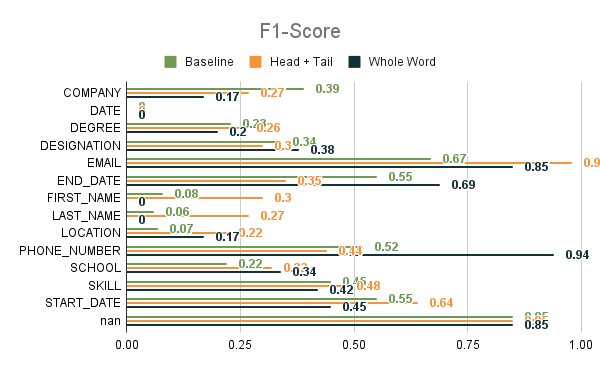
\includegraphics[width=\columnwidth]{comparison_chart.png}
    \caption{%
      Comparison of F-score values for each label across the different feature
      sets.
    }
    \label{figure:2}
  \end{figure}
  \begin{figure}[ht!]
    \centering
    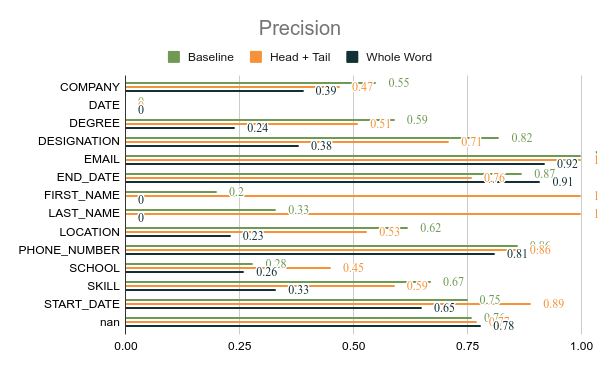
\includegraphics[width=\columnwidth]{p_comparison_chart.png}
    \caption{%
      Comparison of precision values for each label across the different feature
      sets.
    }
    \label{figure:3}
  \end{figure}
  \begin{figure}[ht!]
    \centering
    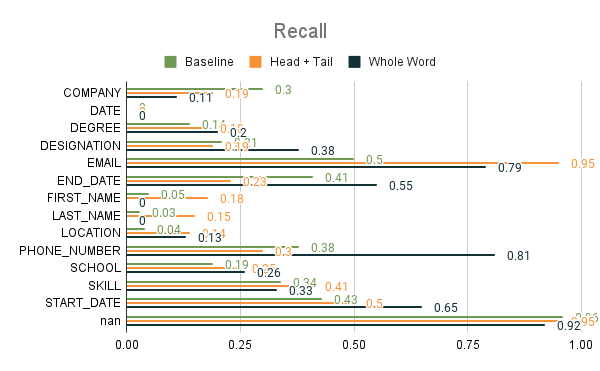
\includegraphics[width=\columnwidth]{r_comparison_chart.png}
    \caption{%
      Comparison of recall values for each label across the different feature
      sets.
    }
    \label{figure:4}
  \end{figure}


% Capítulo 7

\chapter{Conclusions} % Main chapter title

\label{Cap7} % For referencing the chapter elsewhere, use \ref{Chapter1} 

\lhead{Capítulo 6. \emph{Conclusions}} % This is for the header on each page - perhaps a shortened title

  Natural Language Processing is one of the most challenging tasks when it
  comes to artificial intelligence. However, that doesn't mean that there is no
  way to surmount these challenges. With a large enough dataset, it is easier
  for the model to detect certain patterns in our language. Alternatively, this
  kind of model benefits from access to a specific database for skills, names,
  and other proper nouns. Even without these benefits, this CRF is a great
  fundamental step in the right direction for processing resumes automatically. 

  The amount of quality data available is one of the most important parts of
  training any kind of model. In previous works, we have seen the best
  performance when the most amount of data is available. For instance,
  Ayishathahira et. al \cite{Ayishathahira2018a} had a dataset of 800 curated
  resumes and they were able to beat traditional deep learning methods with
  their CRF model. Even when we look at the different feature sets, the one
  with the best performance is also the one with the most amount of samples.
  This project can be taken a step further by collecting a large Spanish resume
  dataset. This would allow the CRF model to better understand certain nuances
  of our natural language.

  It would have been beneficial to have auxiliary datasets with common
  instances of certain entities. E, Suhas & E, Manjunath \cite{E*2020} were
  able to feed a database of known skills to their CRF and as a result, it
  improved the model's performance. In our case, the model would have benefited
  from a database of common Spanish names to increase its performance in
  detecting people's names. The same could have been done for locations if the
  model was trained for a more geographically restricted zone. For some
  entities, it is necessary to have the extra context to help the model learn
  better.

  Regardless of the shortcomings, this model is a great basis for further work
  in the area. Since the model is good at discriminating essential resume
  information, it would already serve as a great tool to reduce the volume of
  data that recruiters and other HR representatives have to parse through. It
  could even be used as part of a parsing pipeline where its output is fed into
  another model to further refine the results. There is a lot of room for
  improvement but we can at least be sure that we are pointing in the correct
  direction.

  There is a lot to gain from teaching computers to understand our language.
  The delegation of tedious and time-consuming work to automated models can
  free people to invest time in more complex and rewarding tasks. This project
  aimed to create a tool that could help people ease their workload, and to
  some extent, we were able to achieve that goal. We can only hope that, based
  on this research, others can build even more powerful tools and improve the
  collaboration between humans and automated systems. 



%----------------------------------------------------------------------------------------
%	THESIS CONTENT - APPENDICES
%----------------------------------------------------------------------------------------

\addtocontents{toc}{\vspace{2em}}

\appendix % Cue to tell LaTeX that the following 'chapters' are Appendices

% Include the appendices of the thesis as separate files from the Appendices folder


% % Appendix A

\chapter{Código Relevante} % Main appendix title

\label{ApenA} % For referencing this appendix elsewhere, use \ref{AppendixA}

\lhead{Apendice A. \emph{Código Relevante}} % This is for the header on each page - perhaps a shortened title
  %modificame si not tienens apendices comenta esta linea

\addtocontents{toc}{\vspace{2em}}

\backmatter

%----------------------------------------------------------------------------------------
%	BIBLIOGRAPHY
%----------------------------------------------------------------------------------------
\label{Bibliography}

\lhead{\emph{Bibliography}}
\bibliographystyle{unsrt}
\bibliography{library, other}
\end{document}
